\subsection{Pythonic Idioms}
\label{idioms}
Using the methodology described in section~\ref{methodology}, we picked the top 10 most popular python idioms from work of Alexandru et al.~\cite{Alexandru2018} and compared Copilot suggestions when prompted with a input method~(shown in section~\ref{input}) and evaluated using methodology shown in section~\ref{evaluation}. 

Copilot suggested the idiomatic approach as the first suggestion in 2 of the 10 idioms we tested i.e., 2 out of 10 instances Copilot had the recommended way as its top suggestion. However, 4 out of those remaining 8 Idioms had the idiomatic way in Copilot's top 10 suggestions. Copilot did not have the idiomatic way in any of its top 10 suggestions for 4 idioms out of 10 idioms we tested.

Table~\ref{tab:all_idioms} shows the list of all the 10 idioms we tested and the ranking of the idiomatic way in Copilot suggestions (if it exists).

\renewcommand{\arraystretch}{1.7}
\begin{table}[ht]
    \centering
    \begin{tabular}{|L|c|}
    \hline
         \textbf{Idiom Title} & \textbf{Copilot Suggestion Matched?} \\
         & (out of 10 suggestions) \\
         \hline
         List comprehension & No \\
         \hline
         Dictionary comprehension & No \\
         \hline
         Mapping & 9\textsuperscript{th} \\
         \hline
         Filter &  7\textsuperscript{th} \\
         \hline
         Reduce & 9\textsuperscript{th} \\
         \hline
         List enumeration & No \\
         \hline
         Set comprehension & 1\textsuperscript{th} \\
         \hline
         Read and print from a file & 5\textsuperscript{th} \\
         \hline
         Add int to all list numbers & No \\
         \hline
         If condition check value & 1\textsuperscript{th} \\
         \hline
    \end{tabular}
    \caption{List of all python idioms tested on Copilot.}
    \label{tab:all_idioms}
\end{table}


Figure~\ref{fig:idioms_1} shows the example of list comprehension idiom, showing user input (i.e., human input), the top suggestion by Copilot and the idiomatic way from Alexandru et al.~\cite{Alexandru2018}.

\begin{figure}[hbt!]
    \centering
    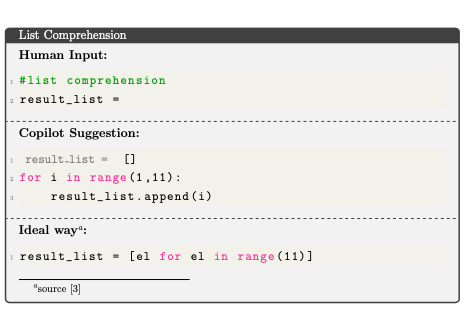
\includegraphics[width=\linewidth]{Figures/idioms_1.png}
    \caption{List Comprehension Idiom and Copilot Suggestion}
    \label{fig:idioms_1}
\end{figure}

The results show that Copilot did not suggest the optimal way as its first suggestion in the majority of the idioms we tested. This shows that current \cct{} like Copilot cannot suggest the idiomatic way in every suggestion even though they are the top most frequently used python idioms in public repositories on GitHub~\cite{Alexandru2018}. 

Copilot being closed source we cannot investigate the potential reasons behind this behavior. However, one plausible explanation for this behavior is that idiomatic ways may not be as frequent as non-idiomatic ways in Copilot's training data of public repositories on GitHub, making the non-idiomatic way rank higher than the idiomatic way.

\cct{} like Copilot should learn to detect idiomatic ways in public repositories and rank them higher than the most frequently used way in public repositories, so that the first suggestion would be the idiomatic way rather than the non-idiomatic way, which is the desirable way for \cct{} like Copilot. For the scope of this thesis, we leave resolving this problem as future work.

% \begin{tcolorbox}[title=List Comprehension,boxsep=.25mm]
%     %https://tex.stackexchange.com/questions/337909/tcolorbox-tcbline-style
% \textbf{Human Input:}
% \begin{lstlisting}[language={Python}]
% #list comprehension
% result_list = 
% \end{lstlisting}
% \tcbline
% \textbf{Copilot Suggestion:}
% \begin{lstlisting}[language=Python,escapechar=\%]
% % \noindent\textcolor{gray}{result\_list  =} % []
% for i in range(1,11):
%     result_list.append(i)
% \end{lstlisting}
% \tcbline
% \textbf{Idiomatic way\footnote{source \cite{Alexandru2018}}:}
% \begin{lstlisting}[language=Python]
% result_list = [el for el in range(11)]
% \end{lstlisting}
% \end{tcolorbox}

%%%%%% TODO: remember to update the screenshot if the source citation is different from the citation in the text %%%%%%

All the Idioms shown in Table~\ref{tab:all_idioms} can be found in the \repl{} including the code used as input (i.e., human input), the top suggestion by Copilot and the idiomatic way suggested in Alexandru et al.~\cite{Alexandru2018}.
